\documentclass[12pt, letterpaper]{article}
\usepackage[utf8]{inputenc}
\usepackage{amsmath}
\usepackage{graphicx}
\graphicspath{ {images/} }

\title{First document}
\author{Sumit Ghosh \thanks{only following the LaTeX tutorials by ShareLaTeX}}
\date{September 2017}

\begin{document}

\maketitle

We have now added a \textbf{title}, \textit{author} and \underline{date} to our first \LaTeX{} document!

In physics, the mass-energy equivalence is stated by the equation $E=mc^2$, discovered in 1905 by Albert Einstein.

The mass-energy equivalence is described by the famous equation

$$E=mc^2$$

discovered in 1905 by Albert Einstein.
In natural units ($c=1$), the formula expresses the identity

\begin{equation}
E=m
\end{equation}

The universe is immense and it seems to be homogeneous, in a large scale, everywhere we look at.

\begin{figure}[h]
	\centering
	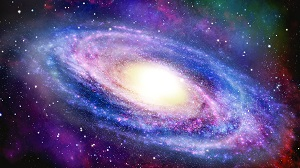
\includegraphics{galaxy}
	\caption{A galaxy}
	\label{fig:mesh1}
\end{figure}

As you can see above, the universe is really beautiful!

\begin{itemize}
		\item The individual entries are indicated with a black dot, a so-called bullet,
		\item The text in the entries may be of any length.
\end{itemize}

\begin{enumerate}
	\item This is the first entry in our list
	\item The list number increases with each entry we add
\end{enumerate}

\end{document}